\documentclass{tufte-handout}

\title{Two-Way ANOVA with Independent Measures \thanks{equal group sizes}}

%\author[The Tufte-LaTeX Developers]{The Tufte-\LaTeX\ Developers}

\date{} % without \date command, current date is supplied


\usepackage{graphicx} % allow embedded images
  \setkeys{Gin}{width=\linewidth,totalheight=\textheight,keepaspectratio}
  \graphicspath{{graphics/}} % set of paths to search for images
\usepackage{amsmath}  % extended mathematics
\usepackage{booktabs} % book-quality tables
\usepackage{units}    % non-stacked fractions and better unit spacing
\usepackage{multicol} % multiple column layout facilities
\usepackage{lipsum}   % filler text
\usepackage{fancyvrb} % extended verbatim environments
  \fvset{fontsize=\normalsize}% default font size for fancy-verbatim environments

\usepackage{pgfplots}
\pgfplotsset{compat=1.12}

% Standardize command font styles and environments
\newcommand{\doccmd}[1]{\texttt{\textbackslash#1}}% command name -- adds backslash automatically
\newcommand{\docopt}[1]{\ensuremath{\langle}\textrm{\textit{#1}}\ensuremath{\rangle}}% optional command argument
\newcommand{\docarg}[1]{\textrm{\textit{#1}}}% (required) command argument
\newcommand{\docenv}[1]{\textsf{#1}}% environment name
\newcommand{\docpkg}[1]{\texttt{#1}}% package name
\newcommand{\doccls}[1]{\texttt{#1}}% document class name
\newcommand{\docclsopt}[1]{\texttt{#1}}% document class option name
\newenvironment{docspec}{\begin{quote}\noindent}{\end{quote}}% command specification environment


\begin{document}

\maketitle% this prints the handout title, author, and date


%\printclassoptions

\begin{marginfigure}[190pt]
  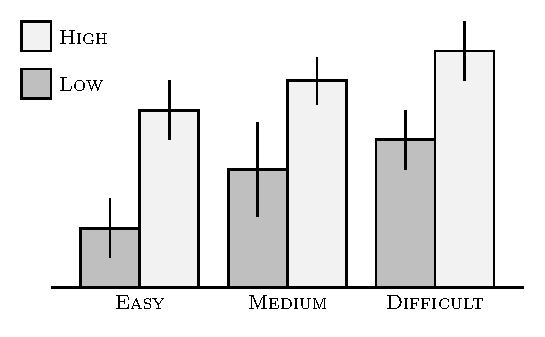
\includegraphics[width=\linewidth]{images/anova_data_two-way}%
  \label{fig:fullfig}%
  \setfloatalignment{t}
\end{marginfigure}

For a two-way experimental design, we consider three separate tests to determine 1) if Factor A has a main effect, 2) if Factor B has a main effect, and 3) if there is an interaction (AxB). Just like the other ANOVAs, these are all F-tests, with slightly different F-ratios

\begin{align*}
F_A&=\frac{SS_A/df_A}{SS_{within}/df_{within}} \qquad
F_B&=\frac{SS_B/df_B}{SS_{within}/df_{within}} \qquad
F_{AxB} &= \frac{SS_{AxB}/df_{AxB}}{SS_{within}/df_{within}}
\end{align*}

\section{Calculating the F-Ratios}
Here, for simplicity, we'll focus on the case where all of the conditions have exactly the same number of participants, which we'll call $r$  (this replaces the sample size $n$). We'll use $a$  and $b$ to denote the number of levels for Factor A and the number of levels for Factor B, respectively. For a 2x3 design, we would have  $a=2$ and $b=3$. With this new notation we have the following $SS$ and $df$ calculations
\begin{align*}
&SS_{between} = r \sum_{\text{groups}} \left( \bar{X}_i - \bar{X}_{all} \right)^2 & &df_{between} = ab-1\\
&SS_{within} = \sum_{\text{groups}} SS_i & &df_{within} = ab(r-1)\\
&SS_A = rb\sum_{\text{levels of A}} \left( \bar{X}_{A_i} - \bar{X}_{all} \right)^2 & &df_A = a-1\\
&SS_B = ra\sum_{\text{levels of B}} \left( \bar{X}_{B_i} - \bar{X}_{all} \right)^2 & &df_B = b-1\\
&SS_{AxB}=SS_{total}-SS_{within}-SS_A-SS_B & &df_{AxB} = (a-1)(b-1)
\end{align*}

\section{Partitioning the Sum of Squares}
Just like the one-way ANOVAs, a helpful tool for understanding these equations is the idea that variability can be \emph{partitioned} into different sources. Here we have two levels of partitioning:
\begin{marginfigure}%
  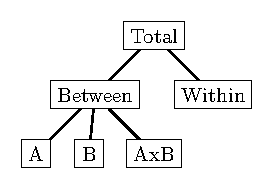
\includegraphics[width=\linewidth]{images/anova_partition_two_way}%
  \label{fig:fullfig}%
  \setfloatalignment{b}
\end{marginfigure}

\begin{align*}
&SS_{total}=SS_{between}+SS_{within} 	&	&df_{total}=df_{between}+df_{within}\\
&SS_{between}=SS_{A}+SS_{B}+SS_{AxB} 	&	&df_{between}=df_{A}+df_{B}+df_{AxB}
\end{align*}

\section{Effect Sizes}
The variance explained for each test is given by

\begin{align*}
&\eta^2_A&=\frac{SS_A}{SS_A+SS_{within}} 	\qquad
&\eta^2_B&=\frac{SS_B}{SS_B+SS_{within}} 	\qquad
&\eta^2_{AxB}&=\frac{SS_{AxB}}{SS_{AxB}+SS_{within}}
\end{align*}


\section{Example}

Suppose you collect data using a 2x3 factorial design with 5 participants in each condition, and observe the data below. What are the values for the test statistics: $F_A$, $F_B$ and $F_{AxB}$?

\begin{table}
  \centering
  \fontfamily{ppl}\selectfont
  \begin{tabular}{llll}
    \toprule
    & Low & Medium & High\\
    \midrule
    Easy & $\bar{X}=3$ & $\bar{X}=5$ & $\bar{X}=10$\\
    & $SS=18$ & $SS=28$ & $SS=26$\\	
    Difficult & $\bar{X}=1$ & $\bar{X}=3$ & $\bar{X}=2$\\
    & $SS=8$ & $SS=20$ & $SS=20$\\	
    \bottomrule
  \end{tabular}
  \label{tab:normaltab}
  %\zsavepos{pos:normaltab}
\end{table}

\vspace{4.5 in}

\begin{table}
  \centering
  \fontfamily{ppl}\selectfont
  \begin{tabular}{lllll}
    \toprule
    Source & \qquad SS & \qquad df & \qquad MS & \qquad F \\
    \midrule
    Between Groups & & & & \\
    \qquad Factor A & & & & \\
    \qquad Factor B & & & & \\
    \qquad Factor AxB & & & & \\
    Within Groups & & & & \\
    Total & & & & \\
    \bottomrule
  \end{tabular}
  \label{tab:normaltab}
  %\zsavepos{pos:normaltab}
\end{table}


\section{Solution}

\begin{fullwidth}
From the description we know that $r=5$. Let's assume that the Easy/Difficult levels correspond to Factor A so that $a=2$, and the Low/Medium/High levels correspond to Factor B so that $b=3$. Once we define our factors, we can find the marginal means (e.g. $\bar{X}_{A_1}, \bar{X}_{A_2}, \cdots$) and grand mean $\bar{X}_{all}$
\end{fullwidth}

\begin{table}
  \centering
  \fontfamily{ppl}\selectfont
  \begin{tabular}{lllll}
    \toprule
    & Low & Medium & High & $\bar{X}_A$\\
    \midrule
    Easy & $\bar{X}=3$ & $\bar{X}=5$ & $\bar{X}=10$ & 6\\
    & $SS=18$ & $SS=28$ & $SS=26$ &\\	
    Difficult & $\bar{X}=1$ & $\bar{X}=3$ & $\bar{X}=2$ & 2\\
    & $SS=8$ & $SS=20$ & $SS=20$ &\\
    \bottomrule
    $\bar{X}_B$ & 2 & 4 & 6 & $\bar{X}_{all}=4$\\	
  \end{tabular}
  \label{tab:normaltab}
  %\zsavepos{pos:normaltab}
\end{table}

\vspace{0.2 in} Now we have all the ingredients to calculate
\begin{align*}
&SS_A = rb\sum_{i} \left( \bar{X}_{A_i} - \bar{X}_{all} \right)^2 = 5 \cdot 3 \left[ (6-4)^2 + (2-4)^2\right] = 120 \qquad \qquad \qquad df_A = a-1 = 2-1 = 1\\
&SS_B = ra\sum_{i} \left( \bar{X}_{B_i} - \bar{X}_{all} \right)^2 = 5 \cdot 2 \left[ (2-4)^2 + (4-4)^2 + (6-4)^2\right] = 80 \qquad df_B = b-1 = 3-1 = 2
\end{align*}

Next, we need to figure out $SS_{between}$ and $SS_{within}$
\begin{align*}
&SS_{between} = r \sum_i \left( \bar{X}_i - \bar{X}_{all} \right)^2 = 5 \left[ (3-4)^2 + (5-4)^2 + (10-4)^2 + (1-4)^2 + (3-4)^2 + (2-4)^2 \right] = 160\\
&SS_{within} = \sum_i SS_i = 18 + 28 + 26 + 8 + 20 + 20 = 120\\
&df_{between} = ab-1 = 2 \cdot 3-1 = 5\\
&df_{within} = ab(r-1) = 2 \cdot 3 (5-1) = 24
\end{align*}

Finally, we can use the partitioning to find $SS_{AxB}$
\begin{align*}
&SS_{AxB}=SS_{total}-SS_{within}-SS_A-SS_B=(160+120)-120-120-80=60\\
&df_{AxB} = (a-1)(b-1) = (2-1)(3-1)=2
\end{align*}

\begin{table}
  \centering
  \fontfamily{ppl}\selectfont
  \begin{tabular}{lrrrl}
    \toprule
    Source &  SS &  df &  MS &  F \\
    \midrule
    Between Groups & 260 & 5 & & \\
    \qquad Factor A & 120 & 1 & 120 & F(1,24)=24 \\
    \qquad Factor B & 80 & 2 & 40 & F(2,24)=8 \\
    \qquad Factor AxB & 60 & 2 & 30 & F(2,24)=6 \\
    Within Groups & 120 & 24 & 5 & \\
    Total & 380 & 29  & & \\
    \bottomrule
  \end{tabular}
  \label{tab:normaltab}
  %\zsavepos{pos:normaltab}
\end{table}

\section{Further Questions}
Are these F-ratios statistically significant? What are the effect sizes?


\end{document}
